\chapter{Architecture Used for Experiments} \label{app:arch}

\def \path {dtcwt_scat}
\def \imgpath {\path/images}

The experiments for this thesis were run on a single server with 8 GPUs and 14
CPUs. The GPUs were each NVIDIA GeForce GTX 1080 cards released in May 2016.
They each have 8GiB of RAM, 2560 CUDA cores and 320 GB/s memory bandwidth.
The CPUs were Intel(R) Xeon(R) E5-2660 models. 

At the completion of the project, we were running CUDA 10.0 with cuDNN 7.6 and 
PyTorch version 1.1.

To do hyperparameter search we used the Tune package \cite{liaw2018tune} which
we highly recommend, as it makes running trials in parallel very easy.

\section{Run Times of some of the Propsed Layers}
.

\chapter{Forward and Backward Algorithms} \label{app:ch3:fwd_bwd}
We have listed some of the forward and backward algorithms here that are not
included in the main text for the interested reader. We also have included 
proofs for the gradients of decimation, interpolation and an entire analysis
decomposition.

\section{Gradients of Sample Rate Changes}\label{sec:app:samplegrads}
Consider 1D decimation and interpolation of a signal $X$. The results we prove
here easily extrapolate to 2D, but for ease we have kept to the 1D case. 

Decimation of a signal $X$ by $M$ is defined as:
\begin{equation}
  Y[n] = X[Mn] \label{eq:app:decimation}
\end{equation}
and interpolation by $M$ as:
\begin{equation}
  Y[n] = \left\{ \begin{array}{ll}
    X[\frac{n}{M}] & n = Mk,\ k\in \integers \\
    0 & \text{otherwise} \\ 
  \end{array}\right.
  \label{eq:app:interpolation}
\end{equation}

\subsection{Decimation Gradient}
From \eqref{eq:app:decimation} the gradient $\dydx{Y_n}{X_k}$ is: 
\begin{equation}
  \dydx{Y_n}{X_k} = \left\{ \begin{array}{ll}
    1 & k = Mn \\
    0 & \text{otherwise} \\
  \end{array} \right.
\end{equation}
By the chain rule, $\dydx{J}{X_k}$ is:
\begin{align}
  \dydx{J}{X_k} &= \dydx{J}{Y_n}\dydx{Y_n}{X_k} \\
                &= \left\{ \begin{array}{ll} 
                \Delta Y[\frac{k}{M}] & k = Mn\\
                  0 & \text{otherwise} \\
                \end{array}\right.
\end{align}
which is interpolating $\Delta Y$ by $M$ from \eqref{eq:app:interpolation}.

\subsection{Interpolation Gradient}
From \eqref{eq:app:interpolation} the gradient $\dydx{Y_n}{X_k}$ is:
\begin{equation}
  \dydx{Y_n}{X_k} = \left\{ \begin{array}{ll}
    1 & n = Mk \\
    0 & \text{otherwise}
  \end{array} \right.
\end{equation}
and then the gradient $\dydx{J}{X_k}$ is:
\begin{align}
  \dydx{J}{X_k} &= \dydx{J}{Y_n}\dydx{Y_n}{X_k} \\
                &= \left\{ \begin{array}{ll} 
                \Delta Y[n] & n = Mk\\
                  0 & \text{otherwise} 
                \end{array}\right. \\
                &= \Delta Y[Mk]
\end{align}
which is decimation of $\Delta Y$ by $M$.
 
\section{Gradient of Wavelet Analysis Decomposition}\label{sec:app:analysis_gradient}
\begin{figure}
  \centering
  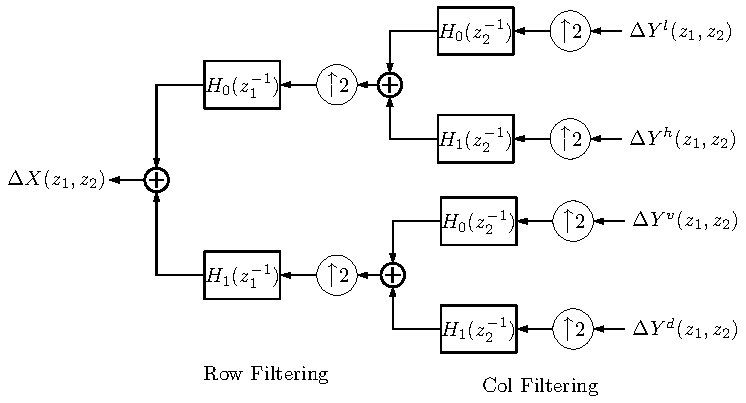
\includegraphics{\imgpath/dwt2d_grad.pdf}
  \mycaption{Gradient of DWT analysis}{Each block in the forward pass of
  \autoref{fig:ch3:dwt} has been swapped for its gradient. The resulting
  gradient has the same form as the inverse DWT.}
  \label{fig:app:dwt_grad_fb}
\end{figure}
We mention in \autoref{sec:ch3:primitives} that the gradient of a forward DWT with
orthogonal wavelets is just the inverse DWT. 
This easily follows from applying the chain rule and using the gradients of each of the
stages of the DWT (convolution becomes correlation, downsampling becomes
upsampling). The equivalent backwards pass of \autoref{fig:ch3:dwt} is
shown in \autoref{fig:app:dwt_grad_fb}.

For an orthogonal wavelet transform, the synthesis filters are the time reverse of
the analysis filters \cite[Chapter 3]{vetterli_wavelets_2007}. This means that
the blocks $H_0(z^{-1}), H_1(z^{-1})$ can be replaced with $G_0(z), G_1(z)$
respectively, giving the inverse DWT.

\section{Extra Algorithms}
In the text we refer to the 2-D inverse DWT which we have listed in
\autoref{alg:ch3:idwt}, as well as the smooth magnitude operation
(\autoref{alg:ch3:mag_smooth}) and the quadratue to complex operation
(\autoref{alg:ch3:q2c}).

\begin{algorithm}[h!]
\caption{2-D Inverse DWT and its gradient}\label{alg:ch3:idwt}
\begin{algorithmic}[1]
\Function{AG:IDWT:FWD}{$ll,\ lh,\ hl,\ hl,\ g_0,\ g_1,\ mode$}
  \State \textbf{save} $g_0,\ g_1,\ mode$ \Comment{For the backwards pass} \label{line:ch3:idwt_save}
  \State $lo \gets \F{sfb1d}(ll,\ lh,\ g_0,\ g_1,\ mode,\ axis=-2) $
  \State $hi \gets \F{sfb1d}(hl,\ hh,\ g_0,\ g_1,\ mode,\ axis=-2) $
  \State $x \gets \F{sfb1d}(lo,\ hi,\ g_0,\ g_1,\ mode,\ axis=-1) $
  \State \textbf{return} $x$
\EndFunction
\end{algorithmic}\vspace{10pt}
\begin{algorithmic}[1]
\Function{AG:IDWT:BWD}{$\delta y$}
  \State \textbf{load} $g_0,\ g_1,\ mode$
  \State $ g_0,\ g_1 \gets \F{flip}(g_0),\ \F{flip}(g_1) $\Comment{flip the filters as in \eqref{eq:ch3:backprop}}
  \State $\Delta lo,\ \Delta hi \gets \F{afb1d}(\delta y,\ g_0,\ g_1,\ mode,\ axis=-2)$ 
  \State $\Delta ll,\ \Delta lh \gets \F{afb1d}(\Delta lo,\ g_0,\ g_1,\ mode,\ axis=-1)$ 
  \State $\Delta hl,\ \Delta hh \gets \F{afb1d}(\Delta hi,\ g_0,\ g_1,\ mode,\ axis=-1)$ 
  \State \textbf{return} $\Delta ll,\ \Delta lh,\ \Delta hl,\ \Delta hh$
\EndFunction
\end{algorithmic}
\end{algorithm}

\begin{algorithm}[tb]
\caption{Smooth Magnitude}\label{alg:ch3:mag_smooth}
\begin{algorithmic}[1]
\Function{AG:MAG\_SMOOTH:FWD}{$x,\ y,\ b$}
  \State $b \gets \max(b,\ 0)$
  \State $r \gets \sqrt{x^2 + y^2 + b^2}$
  \State $\dydx{r}{x} \gets \frac{x}{r}$
  \State $\dydx{r}{y} \gets \frac{y}{r}$
  \State \textbf{save} $\dydx{r}{x},\ \dydx{r}{x}$
  \State \textbf{return} $r - b$
\EndFunction
\end{algorithmic}\vspace{10pt}
\begin{algorithmic}[1]
\Function{AG:MAG\_SMOOTH:BWD}{$\Delta r$}
  \State \textbf{load} $\dydx{r}{x},\ \dydx{r}{y}$
  \State $\Delta x \gets \Delta r \dydx{r}{x}$
  \State $\Delta y \gets \Delta r \dydx{r}{y}$
  \State \textbf{return} $\Delta x,\ \Delta y$
\EndFunction
\end{algorithmic}
\end{algorithm}

\begin{algorithm}[tb]
\caption{Q2C}\label{alg:ch3:q2c}
\begin{algorithmic}[1]
\Function{MOD:Q2C}{$x,\ y,\ b$}
  \State $b \gets \max(b,\ 0)$
  \State $r \gets \sqrt{x^2 + y^2 + b^2}$
  \State $\dydx{r}{x} \gets \frac{x}{r}$
  \State $\dydx{r}{y} \gets \frac{y}{r}$
  \State \textbf{save} $\dydx{r}{x},\ \dydx{r}{x}$
  \State \textbf{return} $r - b$
\EndFunction
\end{algorithmic}\vspace{10pt}
\end{algorithm}
